\documentclass{article}
\usepackage{graphicx} % Required for inserting images
\title{D2: Specifica dei requisiti}
\author{G06}
\usepackage{fancyhdr}
\usepackage{hyperref}
\usepackage{float}
\newcommand{\myheaderimage}{
\includegraphics[width=2cm]{D3/Images/LogoEasyLib.png}}
\pagestyle{fancy}
\fancyhf{} % Clear the header and footer
\lhead{\myheaderimage} % Place the image in the top right corner
\setlength{\headheight}{3cm} % Adjust the height as needed
\rhead{D2-G06}


\begin{document}

\maketitle
\tableofcontents
\newpage

\section{Scopo del Documento}
Questo documento presente la specifica dei requisito del progetto EasyLib. Per riuscire a descrivere al meglio le specifiche, in questo documento si è deciso di aggiungere al linguaggio naturale delle descrizioni create in Unified Modeling Language (UML), per i vari requisiti funzionali, mentre si è optato per delle tabelle strutturate per i requisiti non funzionale del progetto.

\section{Requisiti Funzionali}
Nel presente vengono riportati i requisiti funzionali del sistema utilizzando lo Use Case Diagram in UML e il linguaggio naturale.

\subsection{Registrazione}

\begin{figure}[H]
    \centering
    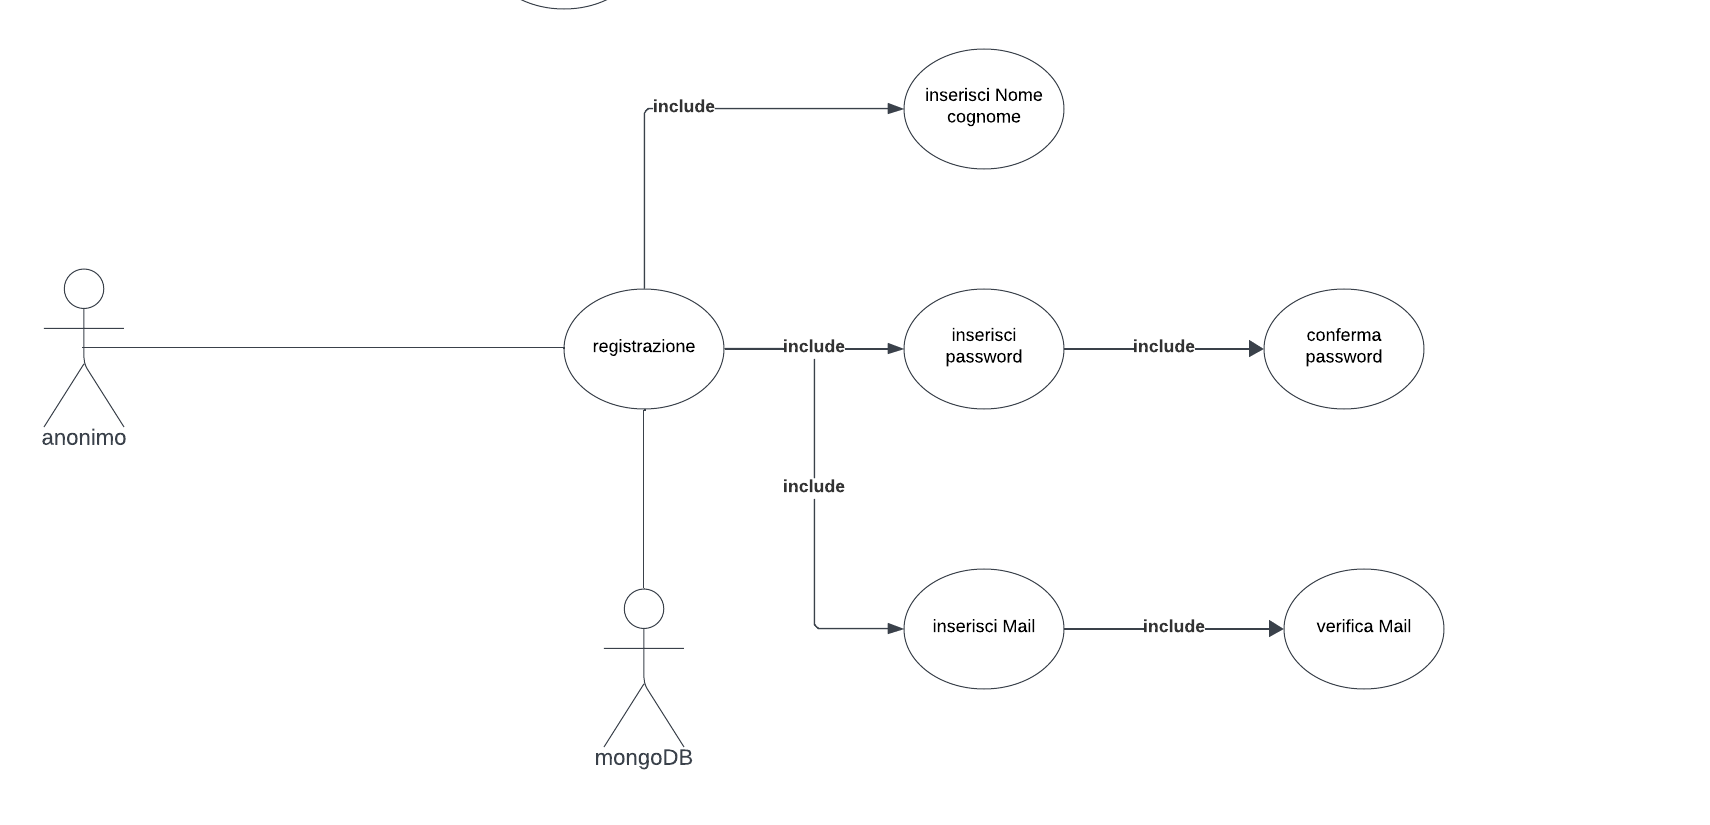
\includegraphics[width=130mm]{D2/Images/registrazioneUML.png}
    \caption{Schema UML registrazione}
\end{figure}
\footnote{Per visualizzare le foto con una qualità maggiore si visiti il seguente link \url{https://drive.google.com/drive/folders/1vMrWNuTA-iFcsAJZy5D8MfoO6Wl2w698?usp=sharing}}
    \underline{Descrizione Use Case "Si registra"}\\
    \textbf{Titolo}: Si registra\\
    \textbf{Riassunto}: Questo use case descrive come avviene l'intero processo di registrazione dell'utente che porta alla creazione di un nuovo account\\
    \textbf{Descrizione}
    \begin{enumerate}
        \item L'utente anonimo clicca il pulsante 'registrati' dalla schermata di login per procedere con la creazione dell'account
        \item L'utente anonimo inserisce nome, cognome mail e password [exception 1]
        \item Il sistema invierà una mail per la registrazione dell'utente [exception 2]
        \item L'utente clicca il link presente nella mail e il sistema comunicherà all'utente l'esito positivo della procedura di registrazione e indirizzerà l'utente alla homepage dell'applicazione EasyLib. [exception 3]
    \end{enumerate}
    \textbf{Exception}
    \begin{itemize}
        \item \textbf{[exception 1]}: Nel caso l'indirizzo mail sia già associato ad un account o password non conforme, il sistema mostrerà un messaggio d'errore all'utente comunicando l'errore e invitando l'utente a inserire mail e/o password diverse.
        \item \textbf{[exception 2]}: Se la mail inserita non è esistente allora non sarà inviata nessuna mail di conferma e sarà mostrato all'utente un messaggio che lo avvisa di dover inserire una mail esistente.
        \item \textbf{[exception 3]}: Se entro 24h l'utente non cliccherà il link presente nell'email, allora la procedura di registrazione fallirà.
    \end{itemize}


    \subsection{Login}
    \begin{figure}[H]
    \centering
    \includegraphics[width=130mm]{D2/Images/loginUML.png}
    \caption{Schema UML login}
\end{figure}

    \noindent\underline{Descrizione Use Case 'Inserisci credenziali'}\\
    \textbf{Titolo}: Inserisci credenziali\\
    \textbf{Riassunto}: Questo use case descrive come avviene l'inserimento delle credenziali per accedere al proprio account.\\
    \textbf{Descrizione}: 
    \begin{enumerate}
        \item L'utente clicca il pulsante login e accede alla pagina login.
        \item L'utente inserisce la propria mail e la propria password [exception 1].
        \item Il sistema conferma l'accesso dell'utente nel proprio account e lo reindirizza alla home dell'applicazione.
    \end{enumerate}
    \textbf{Exception}
    \begin{itemize}
        \item \textbf{[exception 1]}: Nel caso di mail e/o password errate il sistema mostrerà un messaggio di errore all'utente invitandolo a reinserire le proprie credenziali.
    \end{itemize}
    


    \noindent\underline{Descrizione Use Case 'Ripristino password'.}\\
    \textbf{Titolo}: Ripristino password.\\
    \textbf{Riassunto}: Questo use case descrive come avviene il processo di ripristino della password da parte dell'utente.\\
    \textbf{Descrizione}: 
        \begin{enumerate}
        \item L'utente clicca su 'Ripristino password' nel caso in cui abbia dimenticato oppure voglia modificare la propria password
        \item L'utente specifica la propria mail.
        \item Il sistema invierà una mail con un link dove l'utente può modificare la propria  [exception 1].
        \item L'utente inserisce la nuova password [expetion 2]
        \item Il sistema esterno Auth0 gestisce il ripristino della password dell'utente.
    \end{enumerate}
        \textbf{Exception}
    \begin{itemize}
        \item \textbf{[exception 1]}: Se la mail fornita dall'utente è errata verrà mostrato un messaggio d'errore e verrà richiesto all'utente di inserire una mail valida
        \item \textbf{[exception 2]}: Se la nuova password non rispetta i criteri di sicurezza, verrà mostrato un messaggio d'errore e verrà richiesto all'utente di inserire una password valida
    \end{itemize}

    \noindent Questi Use Case sono descritti utilizzando un Activity Diagram
    \begin{figure}[H]
    \centering
    \includegraphics[width=130mm]{D2/Images/activityDiagramLoginRegistrazione.png}
    \caption{Activity Diagram Login e Registrazione}
\end{figure}

    \subsection{Utente autenticato}
\begin{figure}[H]
    \centering
    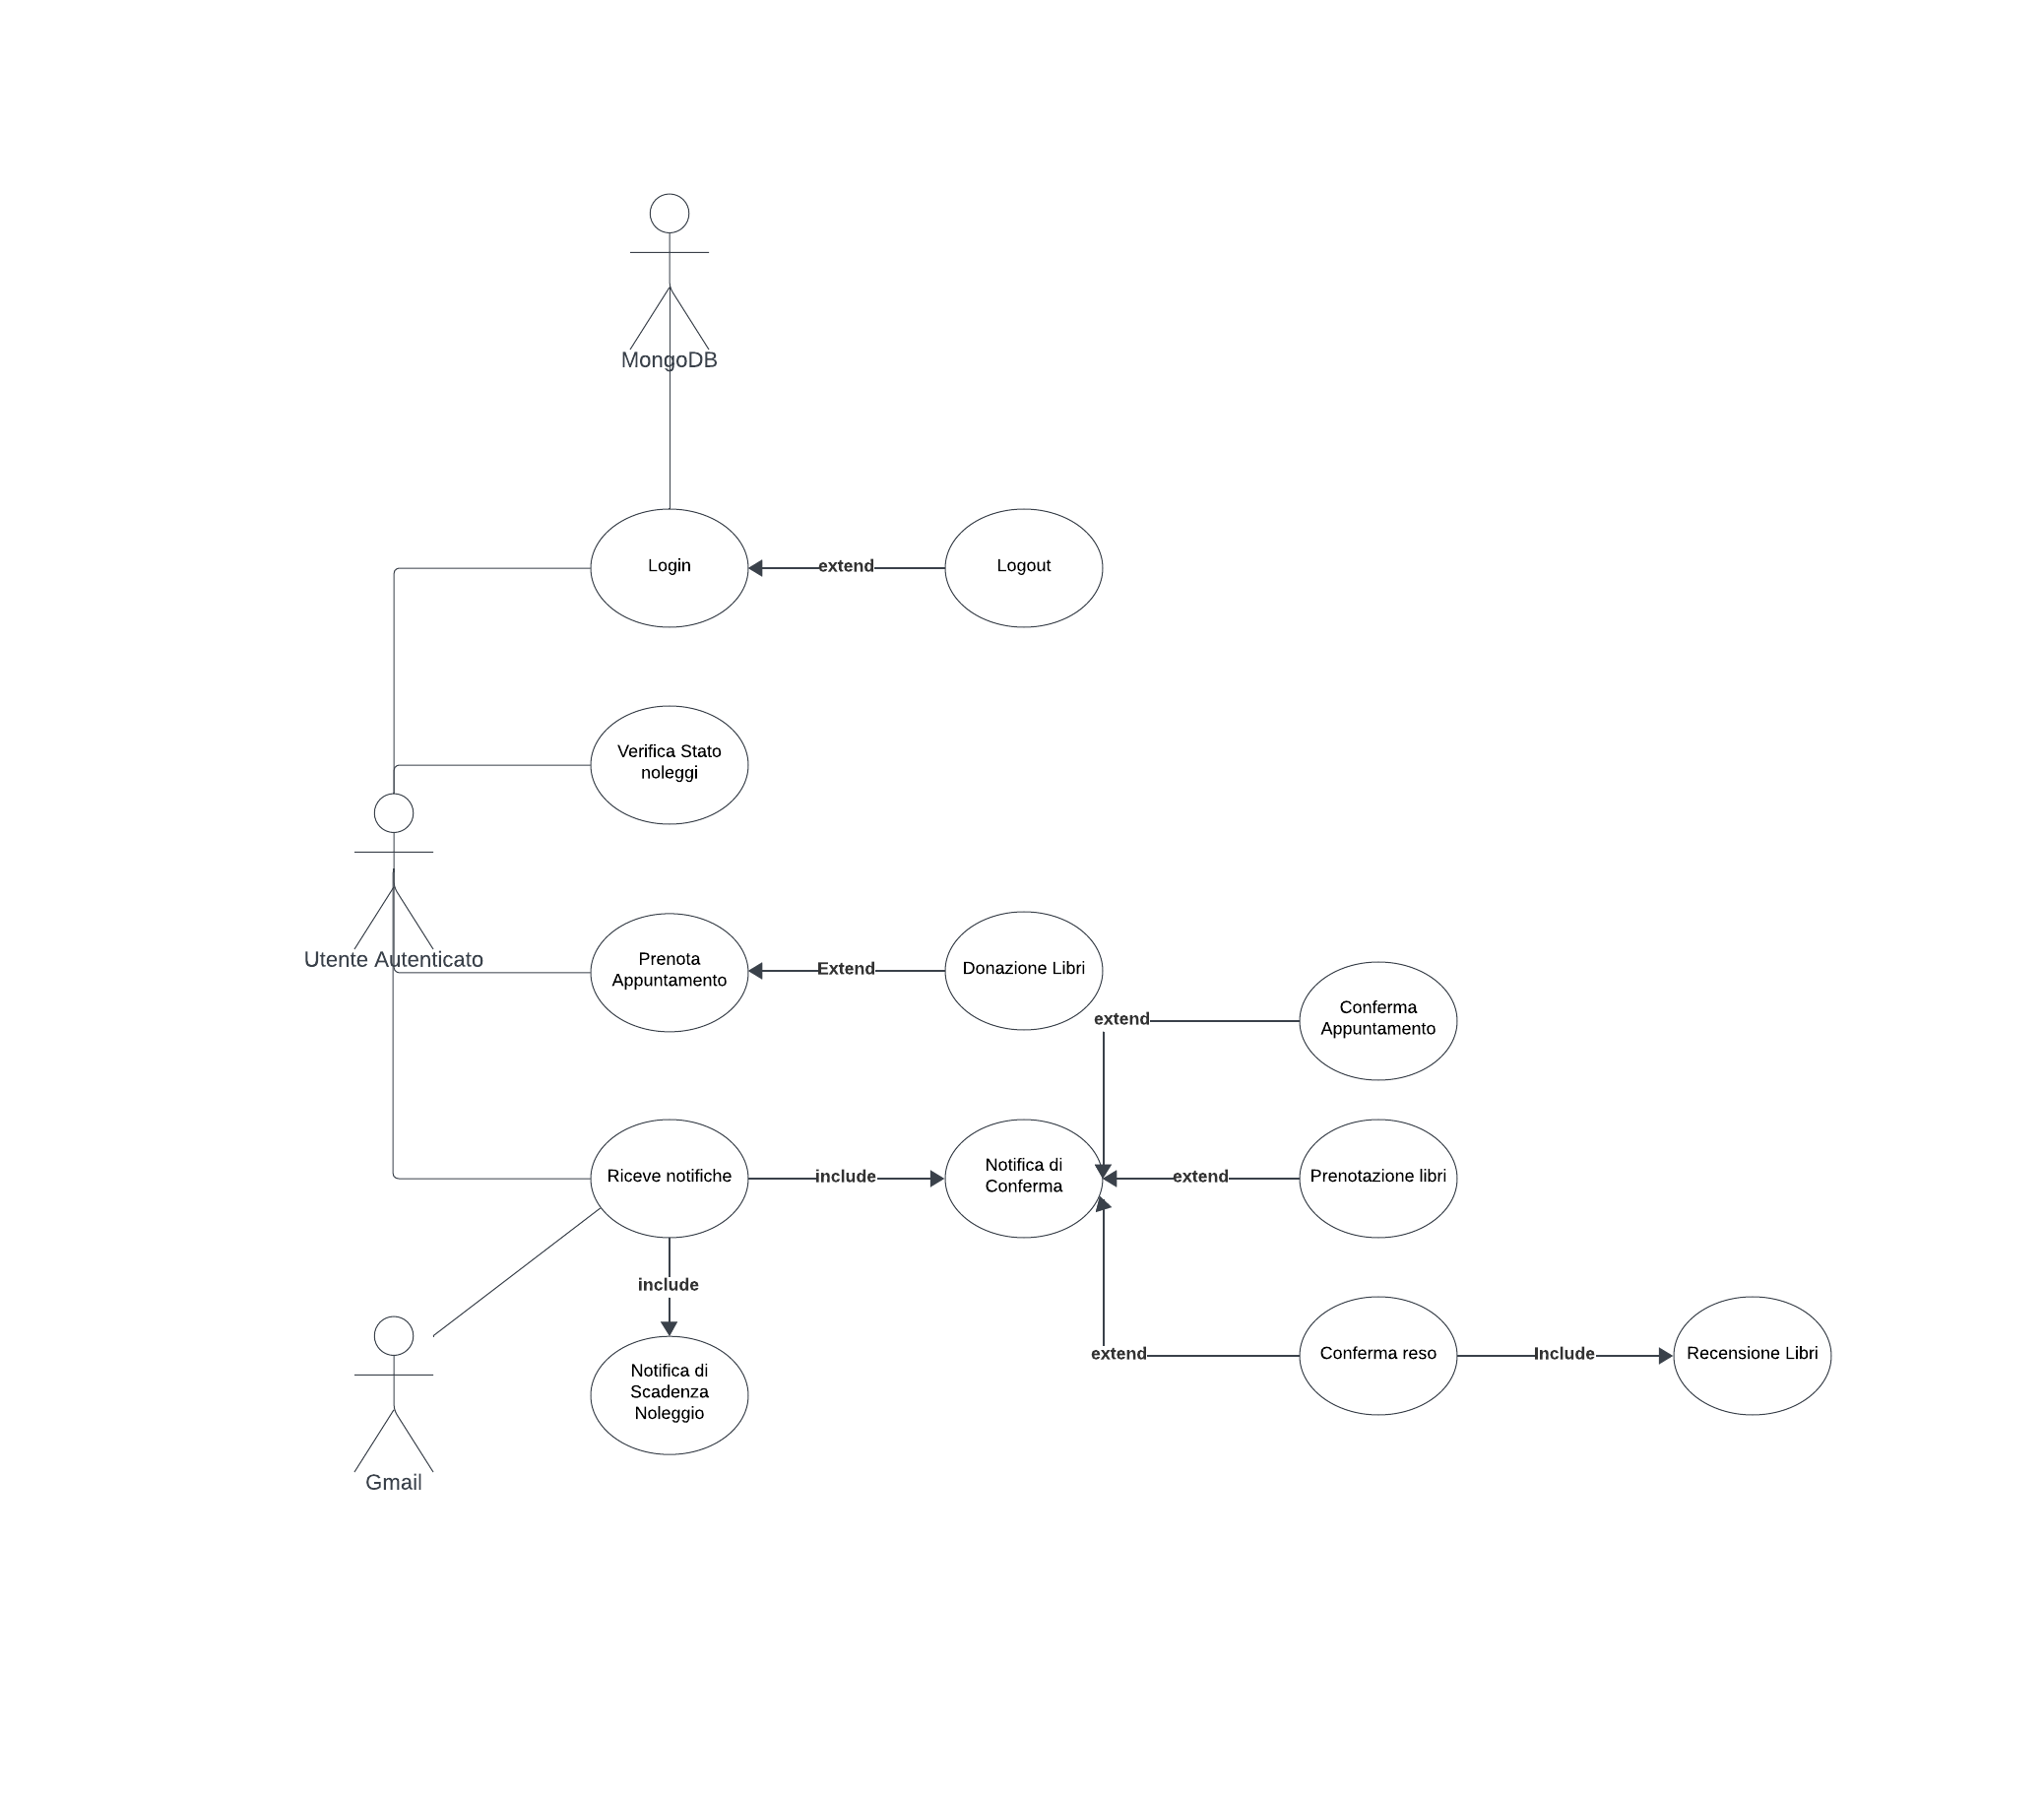
\includegraphics[width=130mm]{D2/Images/UT_autenticato2.png}
    \caption{Schema UML utente autenticato}
\end{figure}

    \noindent\underline{Descrizione Use Case 'Visualizza informazioni personali'.}\\
    \textbf{Titolo}: Visualizza informazioni personali.\\
    \textbf{Riassunto}: Questo use case descrive come avviene la visualizzazione delle informazioni riguardanti il profilo di un utente.\\
    \textbf{Descrizione}: 
        \begin{enumerate}
        \item Dopo aver effettuato l'accesso al proprio profilo, l'utente entra nella sezione impostazioni in modo da vedere le informazioni del proprio profilo
        \item L'utente nelle opportune sezioni, può visualizzare i propri appuntamenti ed eventualmente cancellarli, modificare la propria password, modificare la lingua del sistema, i propri metodi di pagamento, pagare eventuali multe e visualizzare quali libri ha noleggiato.
        \item Il sistema interagisce con il database per leggere/modificare le informazioni.
    \end{enumerate}

    \noindent\underline{Descrizione Use Case 'Modifica Pagamento'}\\
    \textbf{Titolo}: Modifica pagamento\\
    \textbf{Riassunto}: Questo use case descrive come l'utente può modificare i propri metodi di pagamento\\
    \textbf{Descrizione}: 
        \begin{enumerate}
        \item Dopo aver effettuato l'accesso al proprio profilo, l'utente entra nella sezione 'impostazioni $\rightarrow$ i miei pagamenti' e seleziona l'opzione 'Modifica'
        \item L'utente può decidere se eliminare oppure aggiungere un ulteriore metodo di pagamento[extension 1][extension 2][extension 3]
        \item Il sistema poi accede al database per poter modificare il metodo di pagamento dell'utente.
    \end{enumerate}
    \textbf{Extension}: 
        \begin{itemize}
            \item \textbf{[extension 1]}: L'utente può decidere se collegare il proprio account PayPal.
            \item \textbf{[extension 2]}: L'utente può decidere di inserire una carta di credito specificando nome, cognome associati alla carta, numero di carta di credito, codice di sicurezza e data di scadenza.
            \item \textbf{[extension 3]}: L'utente può eventualmente decidere di scegliere un metodo di pagamento predefinito.
        \end{itemize}

    \noindent\underline{Descrizione Use Case 'Modifica appuntamento'}\\
    \textbf{Titolo}: Modifica appuntamento\\
    \textbf{Riassunto}: Questo use case descrive come l'utente può modificare i propri appuntamenti.\\
    \textbf{Descrizione}: 
    \begin{enumerate}
        \item Dopo aver effettuato l'accesso al proprio profilo, l'utente entra nella sezione 'impostazioni $\rightarrow$ i miei appuntamenti' e seleziona l'opzione 'Elimina' o 'Prenota un Appuntamento'[extension 1]
        \item Il sistema poi accede al database per poter modificare gli appuntamenti prenotati o eliminati.
    \end{enumerate}
    \textbf{Extension}: 
        \begin{itemize}
            \item \textbf{[extension 1]}: L'utente se cliccato su 'Prenota un Appuntamento' deve poi decidere la data dell'appuntamento e la motivazione scegliendo tra 'Restituire un libro', 'Donare un libro' o 'Ritirare un libro'
        \end{itemize}

    \noindent\underline{Descrizione Use Case 'Modifica lingua'.}\\
    \textbf{Titolo}: Modifica lingua.\\
    \textbf{Riassunto}: Questo use case descrive come l'utente può modificare la lingua del sistema.\\
    \textbf{Descrizione}: 
    \begin{enumerate}
        \item Dopo aver effettuato l'accesso al proprio profilo, l'utente entra nella sezione 'impostazioni $\rightarrow$ lingua' dove l'utente può decidere la lingua del sistema tra 'Italiano' e 'Inglese'
        \item Il sistema ricaricherà l'applicazione la quale ora sarà nella lingua scelta dall'utente .
    \end{enumerate}

    \noindent\underline{Descrizione Use Case 'Modifica password'}\\
    \textbf{Titolo}: Modifica password\\
    \textbf{Riassunto}: Questo use case descrive come l'utente può modificare la propria password.\\
    \textbf{Descrizione}: 
    \begin{enumerate}
        \item Dopo aver effettuato l'accesso al proprio profilo, l'utente entra nella sezione 'impostazioni $\rightarrow$ account' e clicca su 'Modifica Password'.
        \item L'utente viene reindirizzato ad un form dove poter modificare la password.
        \item l'utente inserisce la password attuale e due volte la nuova password [exception 1]
        \item L'utente viene reindirizzato alla 'homepage' del sistema
        \item Il sistema esterno Auth0 gestisce e salva il cambiamento della password.
    \end{enumerate}
        \textbf{Exception}: 
        \begin{itemize}
            \item \textbf{[exception 1]}: Se la password inserita non sia conforme con i requisiti di sicurezza, il sistema mostra un messaggio d'errore e inviterà l'utente ad inserire una nuova password.
        \end{itemize}

 \noindent\underline{Descrizione Use Case 'Visualizza noleggi'}\\
    \textbf{Titolo}: Visualizza noleggi\\
    \textbf{Riassunto}: Questo use case descrive come l'utente può visualizzare i propri noleggi.\\
    \textbf{Descrizione}: 
    \begin{enumerate}
        \item Dopo aver effettuato l'accesso al proprio profilo, l'utente entra nella sezione 'impostazioni $\rightarrow$ i miei noleggi' per poter vedere i noleggi dei propri libri [extension 1]
    \end{enumerate}
    \textbf{Extension}
    \begin{itemize}
        \item \textbf{[extension 1]}: L'utente può scegliere quale libro tra quelli attualmente noleggiati vuole effettuare il reso. In questo caso clicca il pulsane 'Effettua reso' e una volta fatto ciò gli si aprirà un form dal quale può prenotare un appuntamento per poter restituire il libro.
    \end{itemize}

    \subsection{Utente Amministratore}
    \begin{figure}[H]
    \centering
    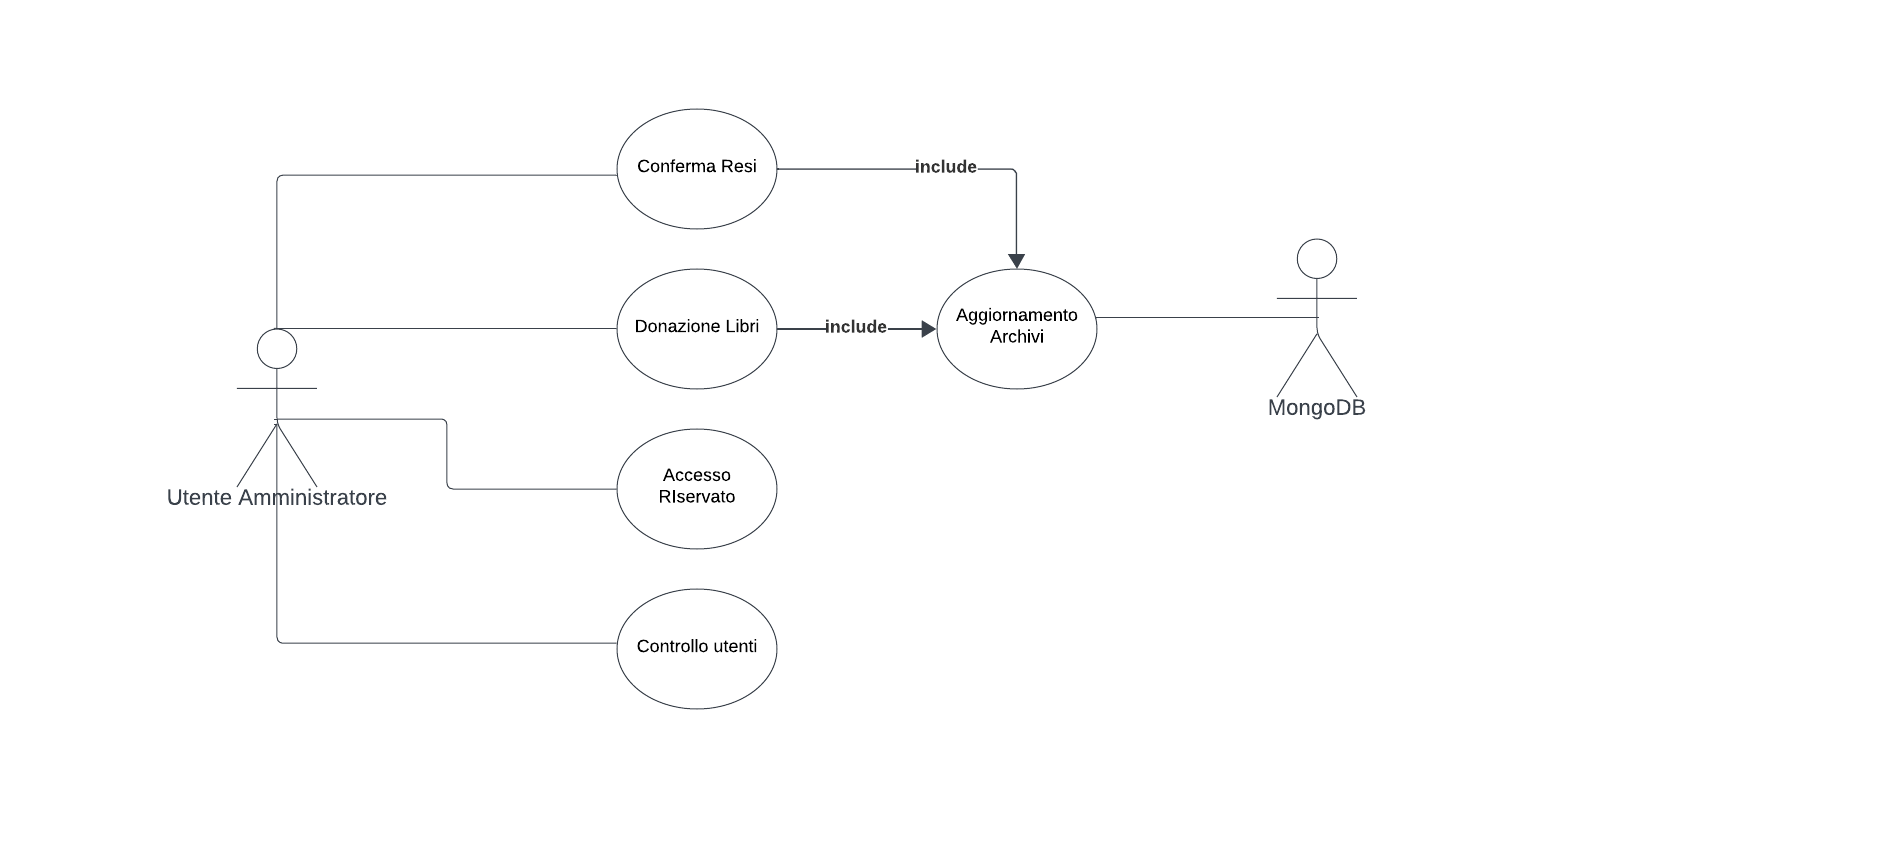
\includegraphics[width=130mm]{D2/Images/Ut_Admin.png}
    \caption{Schema UML utente Admin}
\end{figure}

\noindent\underline{Descrizione Use Case 'Visualizza utenti'}\\
    \textbf{Titolo}: Visualizza utenti\\
    \textbf{Riassunto}: Questo use case descrive come l'amministratore può vedere tutti gli utenti presenti nel database 'Utenti'.\\
    \textbf{Descrizione}: 
    \begin{enumerate}
        \item Dopo aver effettuato l'accesso con le proprie credenziali admin, l'amministratore cliccando il bottone 'Utenti' può visualizzare tutti gli utenti presenti nel database [extension 1] [extension 2]
    \end{enumerate}
        \textbf{Extension}
    \begin{itemize}
        \item \textbf{[extension 1]}: L'amministratore cliccando il pulsante 'Apri pagina multe' gli si aprirà un form dal quale può decidere di dare una multa all'utente il quale non ha ancora effettuato il reso di un libro noleggiato anche se la scadenza del reso è passata da più di 24 ore
        \item \textbf{[extension 2]}: L'amministratore cliccando il pulsante 'Apri pagina noleggi' può decidere di confermare che l'utente ha terminato il noleggio restituendo il libro noleggiato.
    \end{itemize}

     \noindent\underline{Descrizione Use Case 'Aggiungi libro'}\\
    \textbf{Titolo}: Aggiungi libro\\
    \textbf{Riassunto}: Questo use case descrive come l'amministratore può aggiungere un libro al database 'Libri'.\\
    Per descrivere questo use case ci siamo serviti di un Activity diagram:
    \begin{figure}[H]
    \centering
    \includegraphics[width=130mm]{D2/Images/activityDiagramDonazione.png}
    \caption{Activity diagram 'Aggiungi libri'}
\end{figure}

    \subsection{Ricerca}
    \begin{figure}[H]
    \centering
    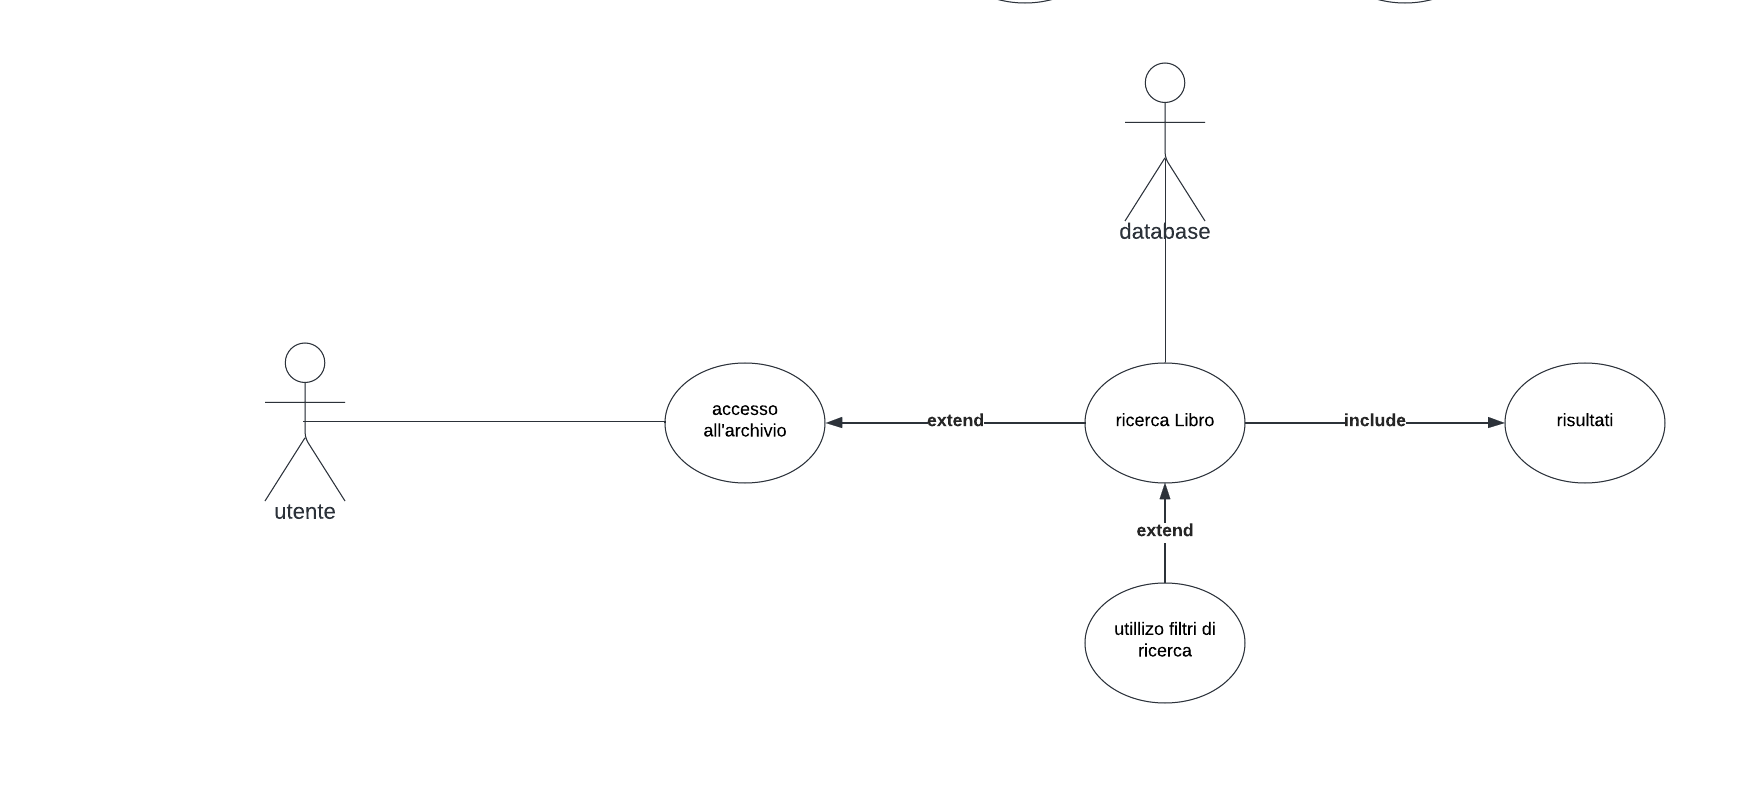
\includegraphics[width=130mm]{D2/Images/ricercaUML.png}
    \caption{Schema UML ricerca}
\end{figure}

\noindent\underline{Descrizione Use Case 'Applica filtro'}\\
    \textbf{Titolo}: Applica filtro\\
    \textbf{Riassunto}: Questo use case descrive come un utente , anonimo o autenticato che sia, può applicare i filtri.\\
    \textbf{Descrizione}: 
    \begin{enumerate}
        \item Dopo essersi recato nella pagina 'Archivio' dell'applicazione l'utente avrà a sua disposizione diversi filtri di ricerca. In particolare potrà selezionare i filtri in base al cognome dell'autore e al genere di proprio interesse.
        \item Scelti i filtri cliccando il pulsante 'Conferma filtri' si aprirà la pagina dei risultati della propria ricerca [exception 1]
    \end{enumerate}
    \textbf{Exception}
    \begin{itemize}
        \item \textbf{[exception 1]}: Se l'utente non seleziona nessun filtro, ma premerà comunque il pulsante 'Conferma filtri' il sistema darà un messaggio d'errore
    \end{itemize}
    
    \noindent\underline{Descrizione Use Case 'Effettua ricerca'}\\
    \textbf{Titolo}: Effettua ricerca\\
    \textbf{Riassunto}: Questo use case descrive come un utente , anonimo o autenticato che sia, possa effettuare la ricerca di un libro presente nell'archivio.\\
    \textbf{Descrizione}: 
    \begin{enumerate}
        \item L'utente inserendo dello parole chiave in uno spazio apposito, la barra di ricerca, potrà ricerca il libro di proprio interesse.
        \item L'utente premerà il tasto 'invio' della propria tastiera[exception 1]
        \item Si caricherà la pagina dei risultati fornendo il risultato della ricerca effettuata
    \end{enumerate}
        \textbf{Exception}
    \begin{itemize}
        \item \textbf{[exception 1]}: Se l'utente preme il tasto 'invio' della propria tastiera pur non avendo inserito nessuna parola chiave, il sistema mostrerà all'utente un messaggio d'errore.
    \end{itemize}

\noindent\underline{Descrizione Use Case 'Noleggia un libro'}\\
    \textbf{Titolo}: Noleggia un libro\\
    \textbf{Riassunto}: Questo use case descrive come un utente autenticato può noleggiare un libro.\\
    \textbf{Descrizione}: 
    \begin{enumerate}
        \item Dopo aver ricercato un libro, l'utente autenticato clicca il pulsante 'Prenota e Ritira' per prenotare un libri.
        \item Si apre il form di prenotazione e l'utente inserisce la propria mail e la data in cui andare a ritirare il libro.
        \item L'utente clicca il pulsante 'Conferma l'appuntamento'
        \item Il sistema invia una mail all'utente confermando la prenotazione del libro. [exception 1]
    \end{enumerate}
    \textbf{Exception}
\begin{itemize}
    \item \textbf{[exception 1]}: Nel caso in cui la prenotazione non vada a buon fine, non verrà inviata nessun mail.
\end{itemize}

\noindent\underline{Descrizione Use Case 'Prenota un appuntamento'}\\
\textbf{Titolo}: Prenota un appuntamento\\
\textbf{Riassunto}: Questo use case descrive come un utente autenticato possa prenotare un appuntamento.\\
\textbf{Descrizione}: 
\begin{enumerate}
    \item L'utente inserisce la propria mail e la data dell'appuntamento
    \item L'utente sceglie una tra le opzioni disponibili ('Donare un libro', 'Restituire un libro', 'Ritirare un libro')
    \item L'utente clicca il pulsante 'Conferma l'appuntamento'
    \item Il sistema invia una mail all'utente confermando l'appuntamento.[exception 1]
\end{enumerate}
\textbf{Exception}
\begin{itemize}
    \item \textbf{[exception 1]}: Nel caso in cui la prenotazione dell'appuntamento non vada a buon fine, non verrà inviata nessun mail.
\end{itemize}

    

    \subsection{Pagamenti}
\begin{figure}[H]
    \centering
    \includegraphics[width=130mm]{D2/Images/pagamentiUML.png}
    \caption{Schema UML pagamenti}
\end{figure}

\noindent\underline{Descrizione Use Case 'Paga multa'}\\
\textbf{Titolo}: Paga multa\\
\textbf{Riassunto}: Questo use case descrive come un utente autenticato possa pagare le proprie multe.\\
\textbf{Descrizione}: 
\begin{enumerate}
    \item L'utente autenticato si reca in 'impostazioni $\rightarrow$ le mie multe' 
    \item L'utente autenticato clicca su 'Paga multa'
    \item Il sistema indirizza l'utente ad una pagina di Paypal dove inserire il proprio [extension 1] e procede col pagamento online
    \item L'utente riceve via mail la conferma dell'abbenuto pagamento e della presa in carica dell'ordine [exception 1]
    \item Il sistema rimuove la multa dal database
\end{enumerate}
\textbf{Exception}
\begin{itemize}
    \item \textbf{[exception 1]}: Nel caso in cui il pagamento non vada a buon fine, non verrà inviata nessun mail.
\end{itemize}


    
    \subsection{Recensione Libri}
\begin{figure}[H]
    \centering
    \includegraphics[width=130mm]{D2/Images/valutazioniUML.png}
    \caption{Schema UML valutazioni}
\end{figure}

\noindent\underline{Descrizione Use Case 'Riceve e visualizza notifica per valutare un libro'}\\
\textbf{Titolo}: Riceve e visualizza notifica per valutare un libro\\
\textbf{Riassunto}: Questo use case descrive come un utente possa valutare un libro.\\
\textbf{Descrizione}: 
\begin{enumerate}
    \item L'utente clicca il link ricevuto nella mail.
    \item L'utente viene reindirizzato ad un form nel quale può valutare un libro noleggiato.
    \item L'utente scrive una breve descrizione del libro.
    \item L'utente fornisce un voto da 1 a 5 del libro appena letto.
\end{enumerate}


\section{Requisiti Non Funzionali}

\subsection{RNF 1: Privacy}
\begin{tabular}{|p{4cm}|p{6cm}|p{4cm}|}
\hline
\textbf{Proprietà} & \textbf{Descrizione} & \textbf{Misura} \\
\hline
\textbf{Regolamento per la protezione dei dati (GDPR)} & I dati personali dell’utente (nome,cognome,profilo) non dovranno essere divulgati in alcun modo e dovranno essere conservati in una forma che consenta l’identificazione degli interessati per un arco di tempo non superiore al conseguimento delle finalità per il quale sono stati trattati. (ART. 5 GDPR) & Conforme \\
\hline
\textbf{Eliminazione dei dati} & Sotto richiesta dell’utente, i dati personali del soggetto dovranno essere eliminati. (GDPR) & Conforme \\
\hline
\end{tabular}



\subsection{RNF 2: Linguaggio}

\begin{tabular}{|p{4cm}|p{6cm}|p{4cm}|}
\hline
\textbf{Proprietà} & \textbf{Descrizione} & \textbf{Misura} \\
\hline
\textbf{Scelta del linguaggio per l’applicazione} & L’applicazione dovrà permettere all’utente di scegliere la lingua con la quale visualizzare i contenuti al suo interno. & L’applicazione consentirà all’utente di scegliere tra la lingua italiana o inglese dalle impostazioni. \\
\hline
\end{tabular}\\

\subsection{RNF 3: Scalabilità}\\

\begin{tabular}{|p{4cm}|p{6cm}|p{4cm}|}
\hline
\textbf{Proprietà} & \textbf{Descrizione} & \textbf{Misura} \\
\hline
\textbf{Utilizzo dell’applicazione con un numero crescente di utenti} & L’applicazione dovrà garantire un utilizzo sincrono di un numero crescente di utenti. & L’applicazione dovrà essere in grado di gestire sincronicamente un numero minore o uguale di 2500 utenti. \\
\hline
\end{tabular}\\\\


\subsection{RNF 4: Prestazioni}\\

\begin{tabular}{|p{4cm}|p{6cm}|p{4cm}|}
\hline
\textbf{Proprietà} & \textbf{Descrizione} & \textbf{Misura} \\
\hline
\textbf{Tempo di risposta dell'applicazione ad una ricerca} & Il tempo massimo di risposta per una ricerca nel database. & Quando l’utente cerca un libro all’interno dell’applicazione, i tempi di risposta e caricamento risultati non devono superare i 3 secondi. \\
\hline
\textbf{Transazione tra una pagina e l’altra} & Il tempo massimo necessario a cambiare pagina all’interno dell’applicazione. & Quando l’utente clicca per cambiare la pagina, il tempo massimo di caricamento dovrà essere di 3 secondi. \\
\hline
\textbf{Tempo di Avvio dell’applicazione} & Il tempo massimo di avvio dell’applicazione su un browser compatibile. & L’applicazione dovrà impiegare non più di 3 secondi per l’avvio. \\
\hline
\end{tabular}\\\\

\subsection{RNF 5: Facilità d'uso}\\

\begin{tabular}{|p{4cm}|p{6cm}|p{4cm}|}
\hline
\textbf{Proprietà} & \textbf{Descrizione} & \textbf{Misura} \\
\hline
\textbf{Comprensione e utilizzo dell’applicazione} & L’applicazione deve essere intuitiva e facile all’uso degli utenti. & L’applicazione dovrà essere utilizzabile da un utente senza esperienza, in tutte le sue funzionalità, entro un tempo massimo di 20 minuti. \\
\hline
\end{tabular}\\\\

\subsection{RNF 6: Compatibilità}\\ 

\begin{tabular}{|p{4cm}|p{6cm}|p{4cm}|}
\hline
\textbf{Compatibilità con Chrome} & L’applicazione dovrà essere compatibile con il browser Chrome. & L’applicazione sarà utilizzabile in tutte le sue funzioni con tutte le versioni di Chrome a partire dal 2023. \\
\hline
\textbf{Compatibilità con Firefox} & L’applicazione dovrà essere compatibile con il browser Firefox . & L’applicazione sarà utilizzabile in tutte le sue funzioni con tutte le versioni di Firefox a partire dal 2023. \\
\hline
\textbf{Compatibilità con Safari} & L’applicazione dovrà essere compatibile con il browser Safari. & L’applicazione sarà utilizzabile in tutte le sue funzioni con tutte le versioni di Safari a partire dal 2023. \\
\hline
\end{tabular}\\\\


\subsection{RNF 7: Sicurezza}\\
 
\begin{tabular}{|p{4cm}|p{6cm}|p{4cm}|}
\hline
\textbf{Proprietà} & \textbf{Descrizione} & \textbf{Misura} \\
\hline
\textbf{Protocollo di trasmissione/ricezione dei dati} & L’applicazione dovrà fornire un livello di sicurezza tale da non permettere agli utenti di accedere ad informazioni di altri utenti. & L’applicazione userà i protocolli HTTPS per il passaggio di dati. \\
\hline

\end{tabular}\\\\



\subsection{RNF 8: Disponibilità}\\



\begin{tabular}{|p{4cm}|p{6cm}|p{4cm}|}
\hline
\textbf{Tempo di Funzionamento} & Il tempo medio espresso in percentuale su un anno solare in cui l’applicazione sarà disponibile all’uso. & La stima è quella che annualmente l’applicazione dovrebbe funzionare senza problemi nel 98\% dei casi. \\
\hline
\textbf{Tempo di Malfunzionamento} & Il tempo massimo, espresso in giorni in un anno solare in cui si pensa che l’applicazione possa riscontrare dei problemi funzionali. & La stima è quella che in un anno l’applicazione possa avere un massimo di 5 giorni complessivi di guasto. \\
\hline

\end{tabular}\\\\


\subsection{RNF 9: Aggiornamenti}\\

\begin{tabular}{|p{4cm}|p{6cm}|p{4cm}|}
\hline
\textbf{Proprietà} & \textbf{Descrizione} & \textbf{Misura} \\
\hline
\textbf{Capacità dell’applicazione di integrare nuovi aggiornamenti} & L’applicazione dovrà essere flessibile ad eventuali aggiornamenti di sistema, tutte le compatibilità non ne dovranno risentire. & A partire dalla versione 1.0 l’applicazione riceverà un minimo di una nuova versione ogni 6 mesi, non intaccando le sue compatibilità con Browser (vedi \textbf{RNF 6}). \\
\hline

\end{tabular}



\subsection{RNF 10: Strong Pass}\\


\begin{tabular}{|p{4cm}|p{6cm}|p{4cm}|}
\hline
\textbf{La password richiesta dall’utente è forte} & L’applicazione richiede all’utente di inserire una password con date specifiche. & La password deve essere composta da: almeno 8 caratteri, di cui almeno uno maiuscolo, inoltre deve contenere almeno un numero e un carattere speciale. \\
\hline

\end{tabular}



\section{Analisi del contesto}
Nel presente verrà discusso il contesto di funzionamento del sistema, prima con una descrizione testuale degli attori ed entità esterne con cui interagisce, poi verrà descritto il flusso di informazioni che scorre tra essi tramite un diagramma di contesto e una sua descrizione a parole.
\textbf{Attori ed entità esterne:}
\begin{itemize}
    \item \textit{Utente:}
    Andrà ad utilizzare il sistema, in particolare  il suo utilizzo si divide in tre tipi in base alla sua tipologia, che può essere:
    \begin{enumerate}
        \item Utente anonimo:
        Andrà ad utilizzare il sistema, ma solo parzialmente, come descritto in RF 2.
        \item Utente autenticato:
        Andrà ad utilizzare il sistema in maniera più completa rispetto all’utente anonimo.
        \item Utente amministratore:
        Utilizzerà una parte specializzata verso la gestione del sistema.
        \end{enumerate}
    \item \textit{MongoDB:}
    È il database su cui vengono salvati l’archivio libri e l’archivio utenti che vengono poi utilizzati dagli utenti descritti sopra.
    \item \textit{Gmail:}
    Sistema che viene utilizzato per la gestione delle notifiche di sistema e credenziali di accesso.
    \item \textit{Google Maps:}
    Fornisce al sistema la mappa che verrà utilizzata nella sezione contatti.
    \item \textit{Paypal:}
    Utilizzato dal sistema per la gestione dei pagamenti delle sanzioni di reso non effettuato entro i limiti di tempo stabiliti.
    \iteml \textit{Auth0}
    Utilizzato dal sistema per la gestione delle credenziali, l'autenticazione quando si esegue il login e il ripristino/modifica della password.
\end{itemize}
Le relazioni delle entità ed attori esterni riguardo al sistema sono:
Utente anonimo, autenticato ed amministratore sono attori; MongoDB è un sistema paritario;
Gmail, Google Maps , Auth0 e PayPal sono sistemi subordinati;

\begin{figure}[H]
    \centering
    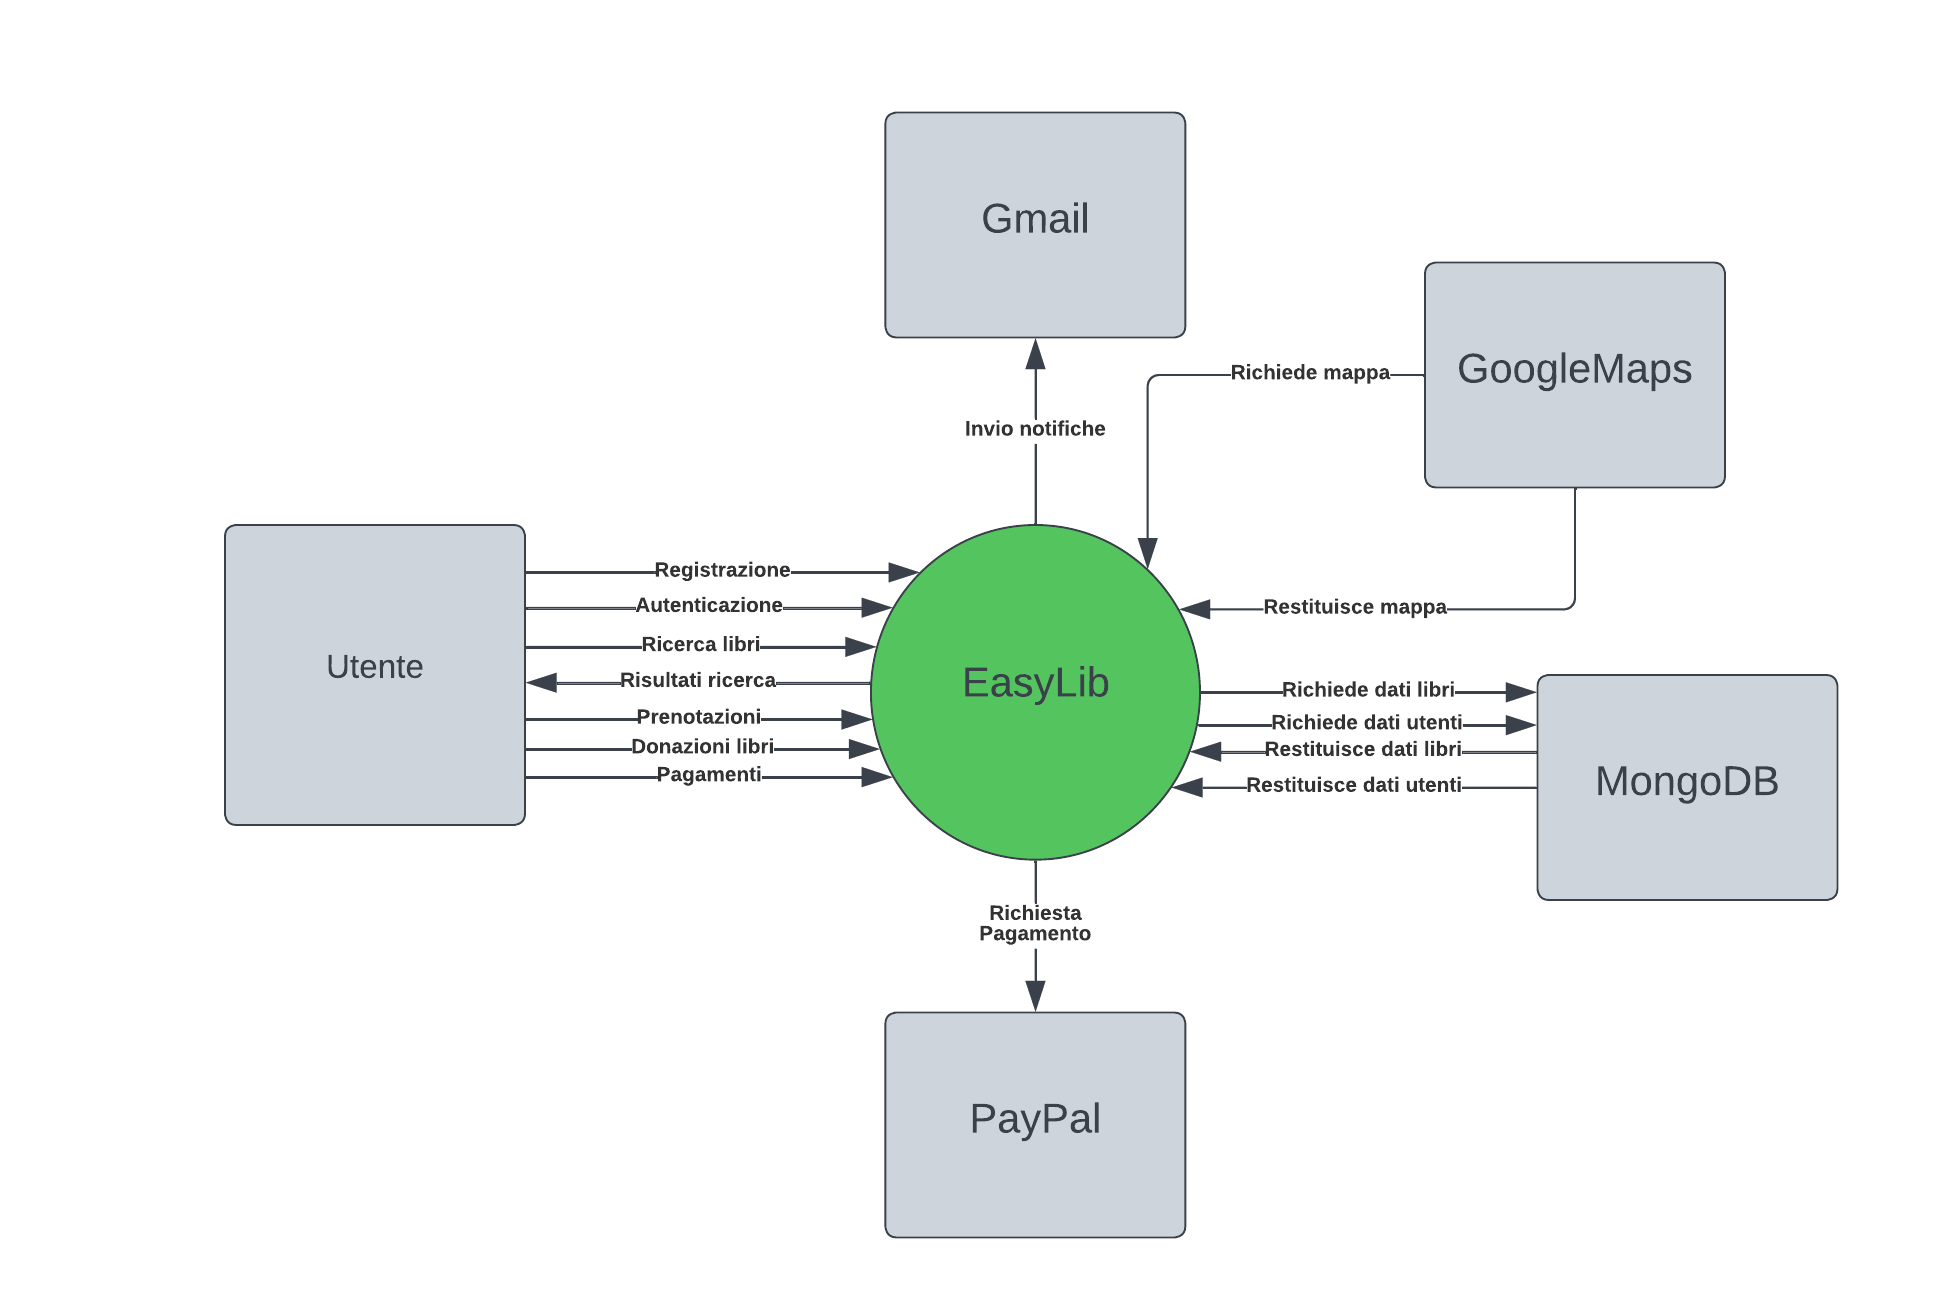
\includegraphics[width=130mm]{D2/Images/Diagramma contesto.png}
    \caption{Diagramma del contesto}
\end{figure}

\section{Analisi dei componenti}
\subsubsection{Diagramma dei componenti:}

\begin{figure}[H]
    \centering
    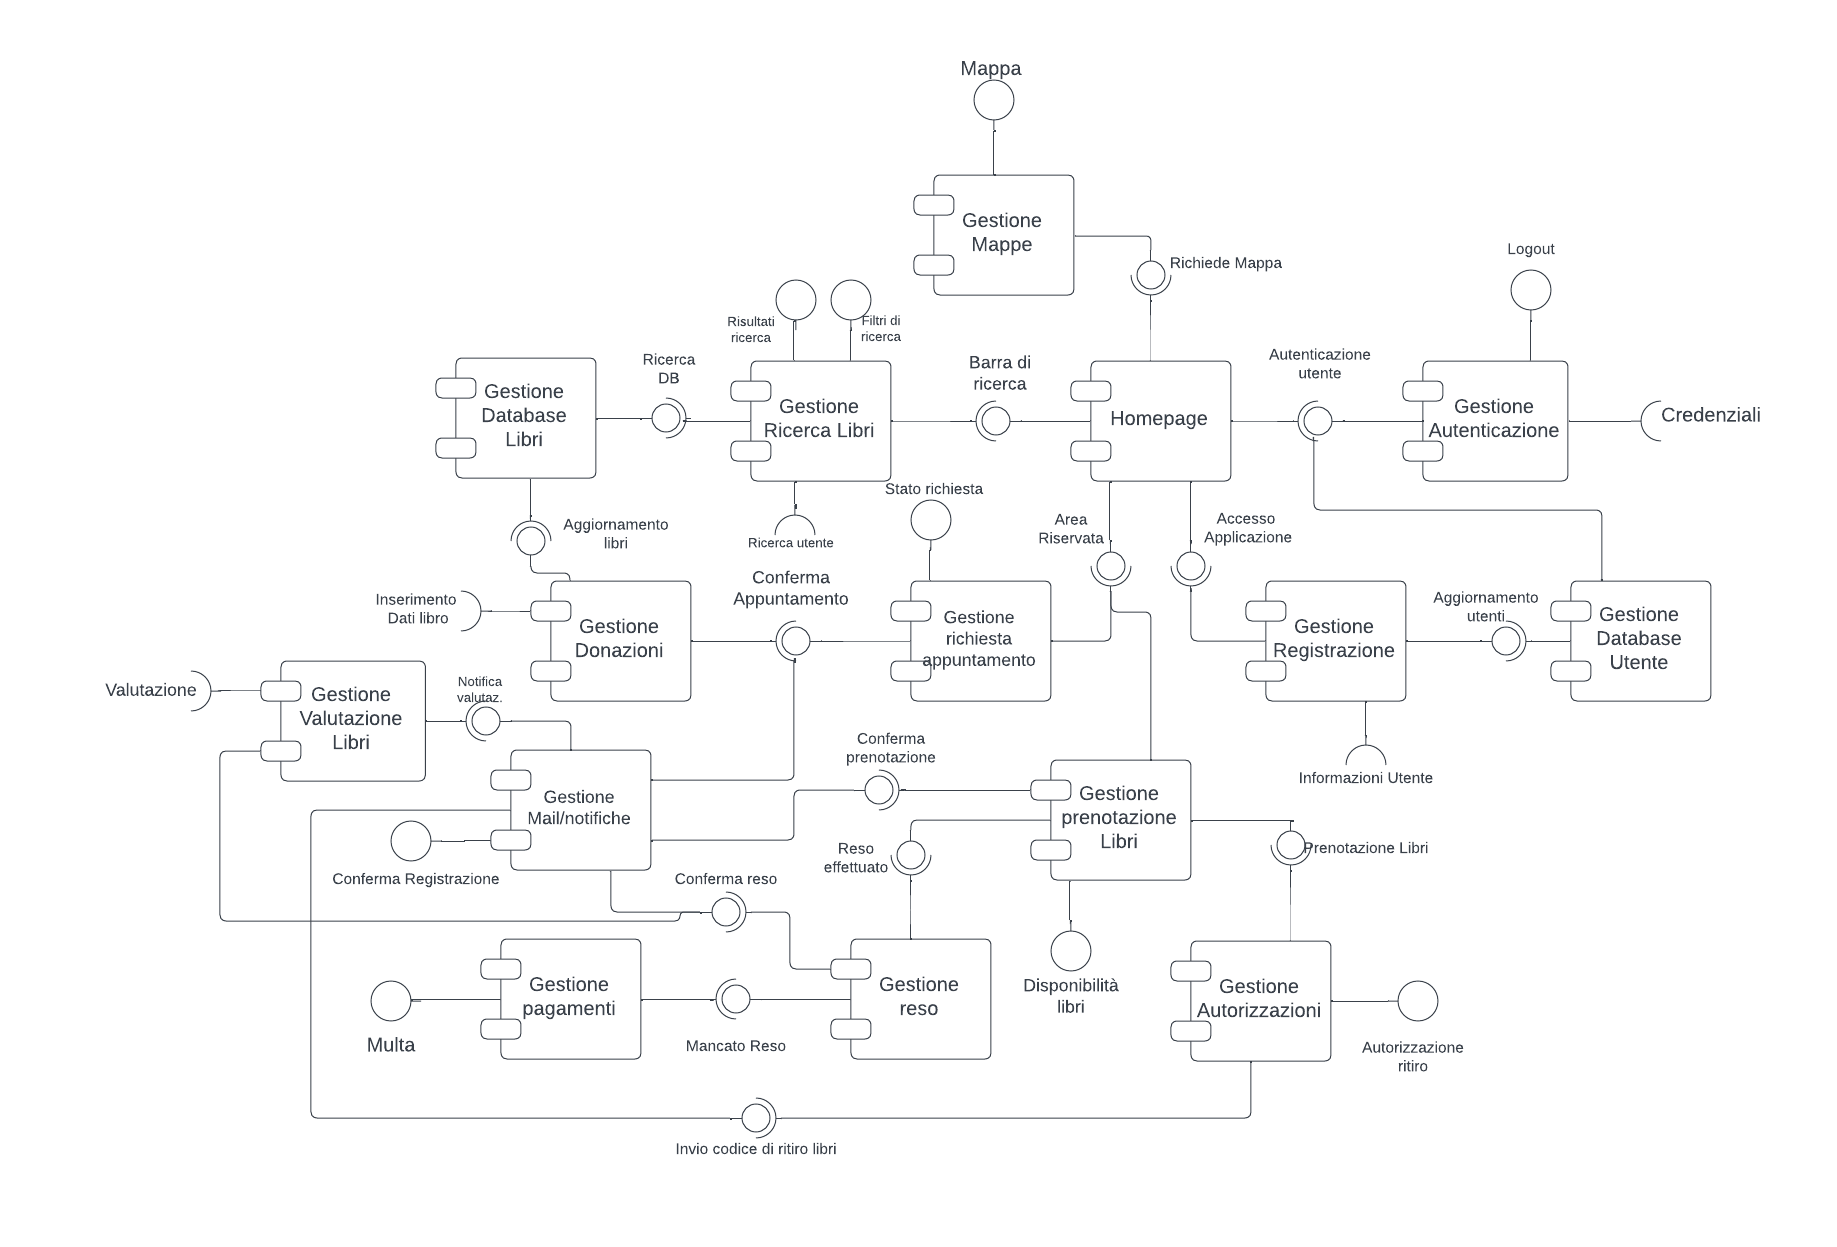
\includegraphics[width=130mm]{D2/Images/Diagramma_componenti_2.png}
    \caption{Diagramma dei componenti}
\end{figure}

\begin{itemize}
    \item \textbf{Gestione ricerca dei libri}
    
    \textit{Descrizione:}Il componente dà la possibilità all’utente di ricercare all’interno del database dei libri specifici tramite un’apposita barra di ricerca.
    \begin{itemize}
        \item \textit{Interfaccia richiesta - Ricerca Database:} Per completare la ricerca e fornire i risultati in output è richiesto l’accesso al database contente i libri in archivio, come specificato nel RF 28.
        \item \textit{Interfaccia richiesta - Barra di ricerca:}La barra di ricerca verrà usata dall’utente per inserire il  libro da cercare in archivio, RF 15.
        \item \textit{Interfaccia richiesta - Input ricerca utente:}L’input è una stringa, ad esempio il titolo di un libro o il nome di un autore, sono richieste all’utente per la ricerca dei libri.
        \item \textit{Interfaccia fornita - Risultati di ricerca:}L’applicazione restituisce l’esito della ricerca fatta dall’utente, accedendo al database e verificando se esiste uno più libri che corrispondono alla ricerca. Se la ricerca non produce risultati verrà inviato un messaggio di errore come specificato nel RF 29.
        \item \textit{Interfaccia fornita - filtri di ricerca:}L’utente può applicare dei filtri che sono forniti dall’applicazione per migliorare i parametri della ricerca e renderla più accurata, vedi RF 16.
         \end{itemize}
    \item \textbf{Gestione autenticazione}
    
    \textit{Descrizione:}Il componente permette all’utente gia registrato di autenticarsi, tramite le credenziali da lui fornite alla prima registrazione, che comprendono una mail e una password con dei requisiti (RNF 10), e accedere alla sua area personale usufruendo di tutte le funzioni dell’applicazione (RF Utente autenticato 3-9). \\
    \begin{itemize}
        \item \textit{Interfaccia richiesta - Credenziali:}L’applicazione richiede dall’utente l’inserimento delle sue credenziali per permettergli l’accesso alla sua area personale, RF 3, se le credenziali non saranno corrette verrà prodotto un messaggio di errore, RF 29.
        \item \textit{Interfaccia fornita - Autenticazione utente:}L’autenticazione avviene tramite un controllo del sistema sul database utenti, in modo tale di garantire un accesso completo al sistema.
        \item \textit{Interfaccia fornita - Logout:} L’utente potrà disconnettersi dalla sua area personale quando vorrà, al suo ritorno dovrà fornire di nuovo le credenziali di accesso.
    \end{itemize}
    \item \textbf{Gestione registrazione}
    
    \textit{Descrizione:}Il componente si occupa della parte di registrazione  utenti, tramite delle informazioni che verranno poi conservate dall’applicazione per la parte di autenticazione.\\
    \begin{itemize}
        \item \textit{Interfaccia richiesta - Informazioni utenti:}Il sistema richiede in input informazioni riguardanti l’utente (nome, cognome, email) e password che verranno utilizzate in seguito per l’accesso autenticato, se i campi avranno degli inserimenti non validi (es. mail non valida, password non rispetta i criteri) verrà restituito un messaggio di errore RF 29 e la registrazione ripartirà da quell’inserimento.
        \item \textit{Interfaccia richiesta - Accesso applicazione:}A seguito della registrazione viene richiesto l’accesso completo al sistema.
        \item \textit{Interfaccia fornita - Aggiornamento database utenti:}A seguito dell’inserimento dati, l’utente viene registrato al sistema aggiornando, con il suo inserimento, il database.
    \end{itemize}
    \item \textbf{Homepage}
    
    \textit{Descrizione:}Il componente rappresenta la prima schermata che l’utente vede al primo accesso sull’applicazione, da qui può decidere se usare l’applicazione come anonimo oppure registrarsi e avere tutte le funzionalità fornite.
    
    \begin{itemize}
        \item \textit{Interfaccia richiesta - Autenticazione utente:}Il componente richiede l’autenticazione degli utenti prima di fornire l’accesso completo al sistema.
        \item \textit{Interfaccia richiesta - Accesso applicazione:}A seguito della registrazione viene richiesto l’accesso completo al sistema.
        \item \textit{Interfaccia richiesta - Richiede mappe:}Il componente richiede la mappa dei punti di ritiro e sedi fisiche di EasyLib.
        \item \textit{Interfaccia fornita - Barra  di ricerca:}Viene fornita una barra di ricerca per effettuare la ricerca dei libri.
        \item \textit{Interfaccia fornita - Area riservata:}Il componente fornisce all’utente l’accesso alla propria area riservata dove ogni utente autenticato potrà visionare lo stato delle proprie operazioni.
    \end{itemize}
    \item \textbf{Gestione richiesta appuntamento}
    
    \textit{Descrizione:}Il componente mostra la parte di richiesta appuntamento all’utente, obbligatoria per poi effettuare donazioni. La componente include anche una parte di conferma appuntamento tramite notifica dall’applicazione.
    
    \begin{itemize}
        \item \textit{Interfaccia richiesta - Area riservata:} Il componente richiede l’accesso all’area riservata.
        \item \textit{Interfaccia fornita - Stato richiesta:} Il componente fornisce la possibilità di visualizzare lo stato delle richieste di appuntamenti.
        \item \textit{Interfaccia fornita - Conferma appuntamento: }L’interfaccia invia una mail tramite il sistema di gestione notifiche per confermare o non,  la data dell’appuntamento scelta dall’utente. 
    \end{itemize}
    \item \textbf{Gestione prenotazione libri:}
    
    \textit{Descrizione:} Il componente gestisce la parte di prenotazione dei libri dell’applicazione. Fornisce anche lo stato di tutti i libri presenti nell’archivio, se sono disponibili al noleggio oppure no, e comprende la prenotazione effettiva del libro.
    
    \begin{itemize}
        \item \textit{Interfaccia richiesta - Area riservata:} Il componente richiede l’accesso all’area riservata.
        \item \textit{Interfaccia fornita - Disponibilità libri:} L’interfaccia fornisce lo stato dei libri presenti sull’applicazione, se sono disponibili al noleggio o meno.
        \item \textit{Interfaccia fornita - Reso:} L’interfaccia fornisce la parte di reso del libro all'utente che include la data di scadenza noleggio e lo stato del reso se è stato confermato o meno(vedi RF 12).
        \item \textit{Interfaccia fornita - Prenotazione libri:} L’interfaccia  fornisce una parte di prenotazione effettiva, in cui il libro può essere riservato e comparirà nel database come non disponibile al noleggio di altri utenti.
        \item \textit{Interfaccia fornita - Invio conferma:} Dopo la prenotazione effettuata, l’applicazione invia una notifica di conferma tramite il sistema mail.
    \end{itemize}
    \item \textbf{Gestione DB libri:}
    
    \textit{Descrizione:} Il componente fornisce l’accesso al database esterno contenente l'elenco dei libri dell’archivio e permette di essere aggiornato dagli utenti amministratori in seguito a donazioni (RF 13).\\
    \begin{itemize}
        \item \textit{Interfaccia fornita - Ricerca DB:} Il componente fornisce la possibilità di cercare all'interno dell’archivio
        \item \textit{Interfaccia fornita - Aggiornamento libri:} Il componente fornisce la possibilità di aggiornare il database di archivio e aggiungere i libri che sono stati donati, all’utente amministratore.
    \end{itemize}
    \item \textbf{Gestione DB utenti}
    
    \textit{Descrizione:} Il componente fornisce l’accesso al database esterno contenente l'elenco degli utenti registrati all'applicazione\\
    \begin{itemize}
        \item \textit{Interfaccia fornita - Aggiornamento utenti:} Il componente permette di aggiornare il database utenti ogni volta che un nuovo utenti si registra all'applicazione.
        \item \textit{Interfaccia fornita - Autenticazione Utente:} L'interfaccia esegue una verifica all’interno del database utente quando un utente già registrato si autentica con le sue credenziali.
    \end{itemize}
    \item \textbf{Gestione donazioni}
    
    \textit{Descrizione:} Il componente viene utilizzato per le parti dell'applicazione che riguardano la donazione libri, tra cui l'inserimento dati del libro (titolo, e autore) e l'inserimento in archivio.
    
    \begin{itemize}
        \item \textit{Interfaccia richiesta - Conferma appuntamento:} Per donare un libro è richiesto l’appuntamento in fisico con un responsabile di Easylib che si occuperà di valutare e inserire il libro nell’applicazione
        \item \textit{Interfaccia richiesta -Inserimento dati libro:} Dopo la donazione è richiesto da parte dell'utente amministratore l’inserimento dei dati del libro donato in archivio.
    \end{itemize}
    \item \textbf{Gestione autorizzazioni}
    
    \textit{Descrizione:} Il componente serve all'applicazione dopo aver ricevuto il messaggio di prenotazione libri, per emettere un codice per l’utente che fornisce l’autorizzazione al ritiro.
    
    \begin{itemize}
        \item \textit{Interfaccia richiesta - Prenotazione Libri:} L’interfaccia richiede che sia già stata fatta la prenotazione libri
        \item \textit{Interfaccia fornita - Autorizzazione ritiro:} L’interfaccia fornisce l’autorizzazione per ritirare il libro dopo che riceve la conferma della prenotazione di un libro.
        \item \textit{Interfaccia fornita - Invio codice di ritiro Libri:} L’interfaccia invia all’utente un codice per il ritiro dei libri da mostrare in fisico tramite la componente mail.
    \end{itemize}
    \item \textbf{Gestione notifiche}\\
    \textit{Descrizione:}Il componente comprende tutte le mail e notifiche che il sistema invia all’utente tramite la mail che viene fornita dall’utente al momento della registrazione.\\
    \begin{itemize}
        \item \textit{Interfaccia fornita - Conferma registrazione:}L’interfaccia invia una mail di conferma registrazione all'utente una volta che la registrazione è terminata con successo.
        \item \textit{Interfaccia fornita - Conferma reso:}L’interfaccia invia una mail di conferma reso all’utente quando l’amministratore ritira il libro dall'utente.
        \item \textit{Interfaccia fornita - Conferma appuntamento:}L’interfaccia invia una mail all’utente per informarlo che la prenotazione è stata fatta con successo, e gli specifica la data in cui è stata fissata.
        \item \textit{Interfaccia fornita -Notifica Valutazione} L’interfaccia invia una mail che permette all'utente di valutare il libro che ha reso. La mail viene inviata 5 giorni dopo che è stata inviata la mail di conferma reso.
        \item \textit{Interfaccia fornita - Conferma prenotazione:}L’interfaccia invia una mail quando la prenotazione di un libro è stata fatta con successo
        \item \textit{Interfaccia fornita - Invio codice di ritiro:}Il componente invia un codice di ritiro all’utente quando la componente di gestione autenticazione autorizza il ritiro
    \end{itemize}
    \item \textbf{Gestione resi:}
    
    \textit{Descrizione:} Il componente serve per tutte le funzionalità di reso previste dall’applicazione, cioè la conferma di reso, il reso effettivo fatto dall’utente in fisico e la parte di mancato reso.
    \begin{itemize}
        \item \textit{Interfaccia richiesta - Reso effettuato:} Il componente richiede che per ogni libro prenotato e in noleggio avvenga il reso, la data di scadenza del noleggio è specificata nell’Homepage di ogni utente.
        \item \textit{Interfaccia richiesta - Conferma reso:} La componente richiede di inviare una mail di conferma reso per ogni volta che un utente ritorna un libro all’archivio.
        \item \textit{Interfaccia fornita - Mancato reso:} Il componente fornisce un interfaccia di mancato reso che viene utilizzata quando un utente non riporta il libro noleggiato.
    \end{itemize}
    \item \textbf{Gestione pagamenti:}
    
    \textit{Descrizione:} Il componente riguarda la parte di pagamenti multe che vengono inviate dopo che un libro non viene riconsegnato, il componente sfrutta l’interfaccia esterna Paypal per ricevere i pagamenti dagli utenti.
    
    \begin{itemize}
        \item \textit{Interfaccia richiesta - Mancato reso:}L’interfaccia richiede che un reso non avvenga nel periodo antecedente alla data di reso, con essa compresa,  prima di emettere una multa nei confronti di un utente.
        \item \textit{Interfaccia fornita - Multa:}L’interfaccia emette una multa che dovrà essere pagata a distanza tramite paypal dall’utente che non ha riportato il libro in tempo, la multa consiste di una cifra simbolica di euro venticinque per ogni reso non effettuato.
    \end{itemize}
    \item \textbf{Gestione Mappe:}

    \textit{Descrizione:} Il componente è usato dall’applicazione per fornire indicazioni geografiche all'utente per permettergli di trovare con più facilità i punti di ritiro
    \begin{itemize}
        \item \textit{Interfaccia fornita - Richiede Mappe:}Il componente fornisce una mappa di tutti i punti di ritiro libri e sedi di EasyLib
    \end{itemize}
    \item \textbf{Gestione Valutazione libri:}
    
    \textit{Descrizione:} Il componente permette all'utente di valutare i libri che ha reso, successivamente dopo aver ricevuto la conferma di reso:
    \begin{itemize}
        \item \textit{Interfaccia richiesta - Valutazione:} l’interfaccia richiede una valutazione da uno a 5 del libro letto dall'utente
        \item \textit{Interfaccia richiesta - Notifica valutazione:} l’interfaccia richiede che sia stata mandata la mail di notifica di valutazione prima di permettere all’utente di valutare il libro.
    \end{itemize}
\end{itemize}





\end{document}